%%%%%%%%%%%%%%%%%%%%%%%%%%%%%%%%%%%%%%%%%%%%%%%%%%%%%%%
% SEZIONE 7 — CONCLUSIONI E SVILUPPI FUTURI
%%%%%%%%%%%%%%%%%%%%%%%%%%%%%%%%%%%%%%%%%%%%%%%%%%%%%%%
\section{Conclusioni e sviluppi futuri}
\label{sec:07_conclusioni}

\epigraph{
    The real voyage of discovery consists not in seeking new landscapes, but in having new eyes.
}{Marcel Proust}

Questo capitolo conclude la tesi riassumendo i principali risultati ottenuti (Paragrafo~\ref{subsec:conclusioni}), per poi delineare le direzioni di ricerca future (Paragrafo~\ref{subsec:sviluppi_futuri}), con una riflessione sul concetto di invariante semantico e sul suo collegamento con la Platonic Representation Hypothesis.

\newpage

%%%%%%%%%%%%%%%%%%%%%%%%%%%%%%%%%%%%%%%%%%%%%%%%%%%%%%%
% SUBSECTION: CONCLUSIONI
%%%%%%%%%%%%%%%%%%%%%%%%%%%%%%%%%%%%%%%%%%%%%%%%%%%%%%%
\subsection{Conclusioni}
\label{subsec:conclusioni}

Il lavoro presentato in questa tesi ha affrontato il problema dell'opacità delle rappresentazioni dense apprese dai modelli linguistici, sviluppando PRISMA, un metodo e un applicativo che scompone gli embedding densi nei concetti atomici che li costituiscono, tramite Sparse Autoencoder.
I risultati sperimentali, presentati nel Capitolo~\ref{sec:06_risultati}, dimostrano l'efficacia dell'approccio su tre livelli.
A livello di singola feature, il SAE estrae direzioni latenti monosemantiche, ciascuna corrispondente a un concetto identificabile e interpretabile. Le Feature 5648 (\textit{Time in physics}) e 1140 (\textit{Ising model}), analizzate in dettaglio, illustrano due regimi complementari: la prima è un concetto \textit{parent}, ampio e pervasivo (densità 15,5\%), radice di una famiglia estesa; la seconda è un concetto \textit{child}, specifico e raro (densità 0,77\%), subordinato a un parent. Entrambe mostrano attivazioni di picco comparabili ($\sim$25), indicando che il SAE assegna intensità elevata sia a concetti generali sia a concetti specifici quando l'input è altamente pertinente.
A livello di organizzazione delle feature, l'algoritmo di clustering gerarchico ha identificato \textbf{590 feature families} sulle oltre 4.000 feature interpretate. Le famiglie presentano una topologia a stella ricorrente, con un parent a semantica ampia e children che ne rappresentano specializzazioni concettuali. La coerenza di queste strutture con le tassonomie dei domini di applicazione, dalla fisica delle particelle alle metodologie del machine learning, conferma che l'organizzazione gerarchica non è imposta dal SAE, ma rivelata da esso.
A livello quantitativo, l'analisi dell'Effective Rank ha dimostrato che la struttura semantica comprime sistematicamente le rappresentazioni. Il Semantic Compression Ratio, metrica originale introdotta in questo lavoro, cresce monotonicamente con l'expansion factor, raggiungendo il \textbf{59,9\%} per $\rho = 64$. Questo risultato è consistente con il fenomeno del feature splitting: all'aumentare della capacità, le feature generali si scindono in sotto-feature più specifiche ma correlate, incrementando il numero di feature nominali senza aumentare proporzionalmente la dimensionalità effettiva.
La correlazione nello spazio dei pesi tra \textit{Ising model} e \textit{Baryon/Boson Spectroscopy} (0.54), discussa nel Paragrafo~\ref{subsubsec:feature_example_ising}, è forse l'esempio più suggestivo emerso da questo lavoro: due domini apparentemente distanti che il SAE colloca in direzioni vicine, riflettendo un'affinità formale, le teorie di campo su reticolo, che un fisico riconosce ma che nessuna tassonomia esplicita aveva codificato. Quando una rete neurale trova connessioni reali ma non ovvie, e un esperto umano le conferma \textit{a posteriori}, è difficile sostenere che la struttura sia un artefatto.

%%%%%%%%%%%%%%%%%%%%%%%%%%%%%%%%%%%%%%%%%%%%%%%%%%%%%%%
% SUBSECTION: SVILUPPI FUTURI
%%%%%%%%%%%%%%%%%%%%%%%%%%%%%%%%%%%%%%%%%%%%%%%%%%%%%%%
\subsection{Sviluppi futuri: verso gli invarianti semantici}
\label{subsec:sviluppi_futuri}

I risultati ottenuti aprono una domanda che va oltre gli obiettivi tecnici del presente lavoro: \textit{PRISMA traduce da una rappresentazione a un'altra. Qual è quella ``vera''?}

\subsubsection{Le ombre sulla parete}
\label{subsubsec:ombre_caverna}
Nel Mito della Caverna, Platone descrive prigionieri incatenati che osservano ombre proiettate su una parete e le scambiano per la realtà. Le ombre sono \textit{proiezioni} di oggetti reali, coerenti, strutturate, predittive, ma non sono gli oggetti stessi.

\begin{figure}[htbp]
    \centering
    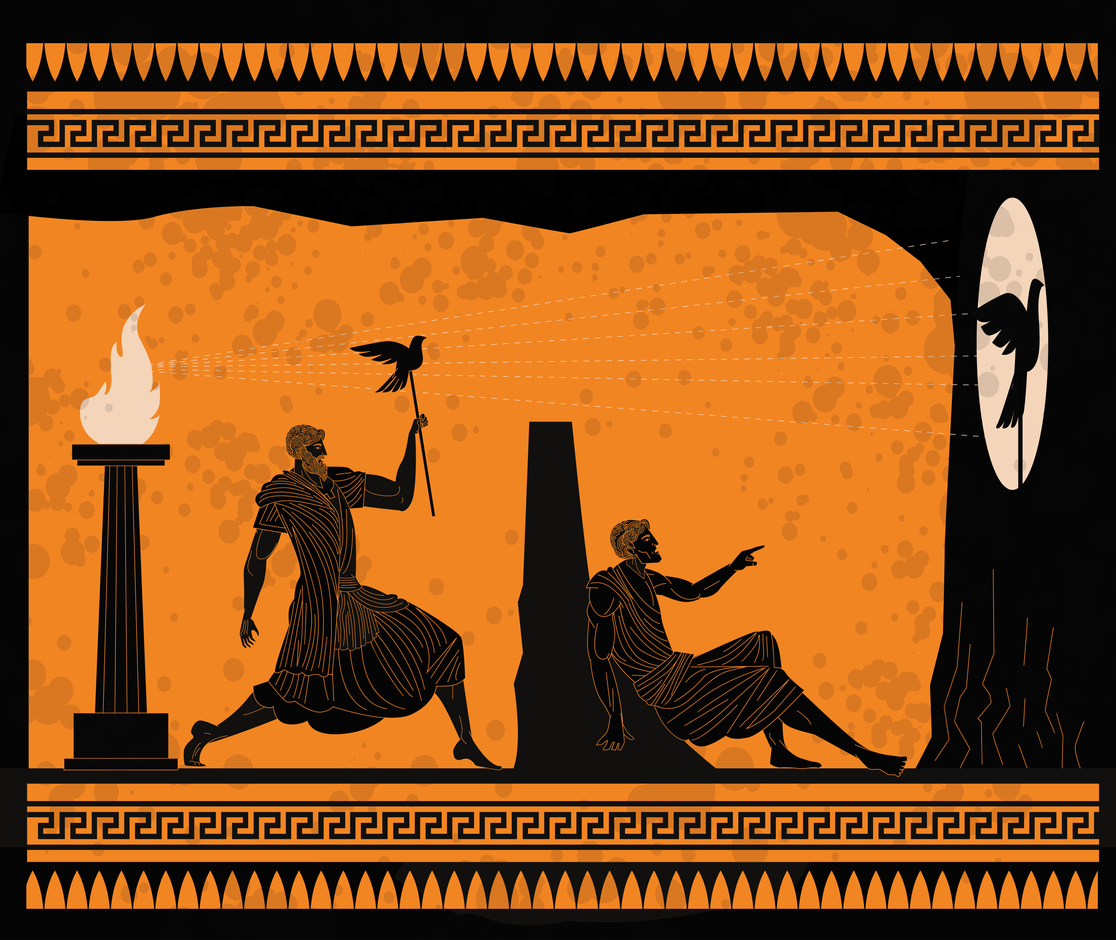
\includegraphics[width=0.85\textwidth]{pictures/cap6/mito_caverna.jpeg}
    \caption{Mito della Caverna di Platone. Un uomo proietta l'ombra di un uccello su una parete; il prigioniero incatenato osserva l'ombra e la scambia per la realtà. La proiezione è coerente, l'ombra ha la forma di un uccello, ma è una riduzione dell'oggetto originale. Nel contesto del presente lavoro, ogni rappresentazione del significato (densa, sparsa, umana) è un'ombra sulla parete: una proiezione strutturata ma parziale di una realtà semantica sottostante. Fonte: \cite{fantaguzzi2024mito}.}
    \label{fig:caverna_platone}
\end{figure}

Nel contesto del presente lavoro, ogni rappresentazione del significato può essere vista come un'ombra sulla parete:

\begin{itemize}
    \item La \textbf{rappresentazione densa} (gli embedding di BERT~\parencite{devlin2018bert} o qualsiasi altro modello sullo stesso paradigma) codifica il significato in vettori $\mathbb{R}^d$ dove ogni dimensione è attiva ma nessuna è interpretabile isolatamente. Il significato emerge dalla combinazione di tutte le dimensioni.
    \item La \textbf{rappresentazione sparsa} (le attivazioni del SAE) codifica lo stesso significato in vettori $\mathbb{R}^n$ dove poche dimensioni sono attive, ciascuna corrispondente a un concetto interpretabile. È la proiezione su cui PRISMA si concentra.
    \item La \textbf{rappresentazione umana}, vale a dire la struttura concettuale con cui viene organizzato il significato, accessibile indirettamente tramite giudizi di similarità, tempi di reazione, errori di memoria e strutture linguistiche, è un'altra proiezione ancora.
\end{itemize}

Tre proiezioni. Tre ombre diverse sulla parete. Ma se preservano le stesse relazioni, se ``re meno uomo più donna uguale regina'' vale nello spazio denso, nello spazio sparso e nella mente umana, allora la domanda diventa: \textit{cosa c'è fuori dalla caverna?}

%%%%%%%%%%%%%%%%%%%%
\subsubsection{La lezione della fisica: non esiste un sistema privilegiato}
\label{subsubsec:lezione_fisica}
La fisica ha affrontato una domanda strutturalmente identica a quella posta alla fine del paragrafo precedente, e la risposta che ha trovato è istruttiva.
\begin{figure}[htbp]
    \centering
    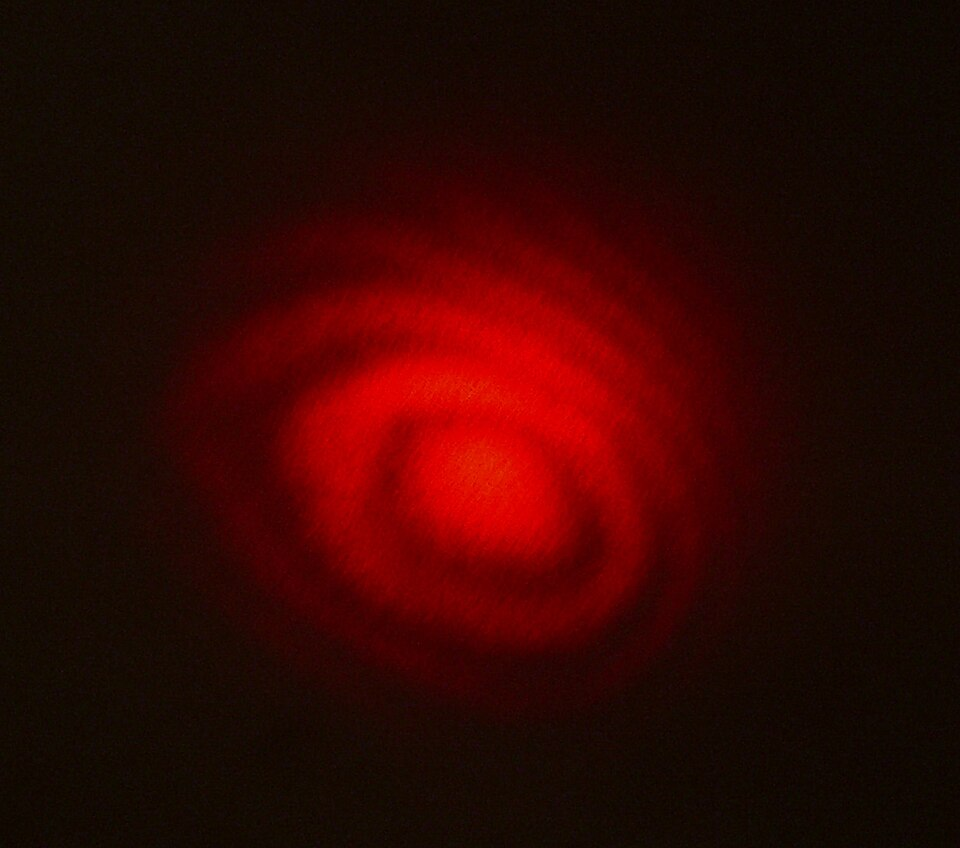
\includegraphics[width=0.6\textwidth]{pictures/cap6/Michelson_Interferometer_Red_Laser_Interference.jpg}
    \caption{Interferenza prodotta da un raggio luminoso rosso con l'esperimento di Michelson-Morley. L'esperimento dimostrò l'indipendenza della velocità della luce rispetto all'ipotetico vento d'etere e costituì la prima forte prova contro la teoria dell'etere luminifero. Eseguito nel 1887 nell'attuale Case Western Reserve University, è considerato uno dei più famosi e importanti esperimenti della storia della fisica. Fonte: \cite{wikipedia2024michelson}.}
    \label{fig:mm_experiment}
\end{figure}
Per gran parte dell'Ottocento, i fisici cercavano l'\textit{etere luminifero}: un mezzo materiale che pervadeva tutto lo spazio e attraverso il quale si propagavano le onde elettromagnetiche. L'etere non era solo un'ipotesi sulla natura della luce: era, implicitamente, un \textbf{sistema di riferimento assoluto}, vale a dire il sistema ``a riposo'' rispetto al quale misurare il moto ``vero'' di tutti gli altri corpi.
Se l'etere esisteva, allora esisteva un modo privilegiato di descrivere la realtà, quello dell'osservatore fermo rispetto all'etere.
L'esperimento di Michelson e Morley (1887) cercò di misurare il moto della Terra rispetto a questo riferimento assoluto, e non trovò nulla. La velocità della luce risultava identica in tutte le direzioni, indipendentemente dal moto dell'osservatore. L'etere, semplicemente, non c'era.

Einstein non risolse il problema dell'etere: lo dissolse. Anziché cercare il riferimento giusto, postulò che \textbf{non ne esiste uno privilegiato}: tutti i sistemi di riferimento inerziali sono equivalenti, e le leggi della fisica assumono la stessa forma in ciascuno di essi.
\begin{figure}[htbp]
    \centering
    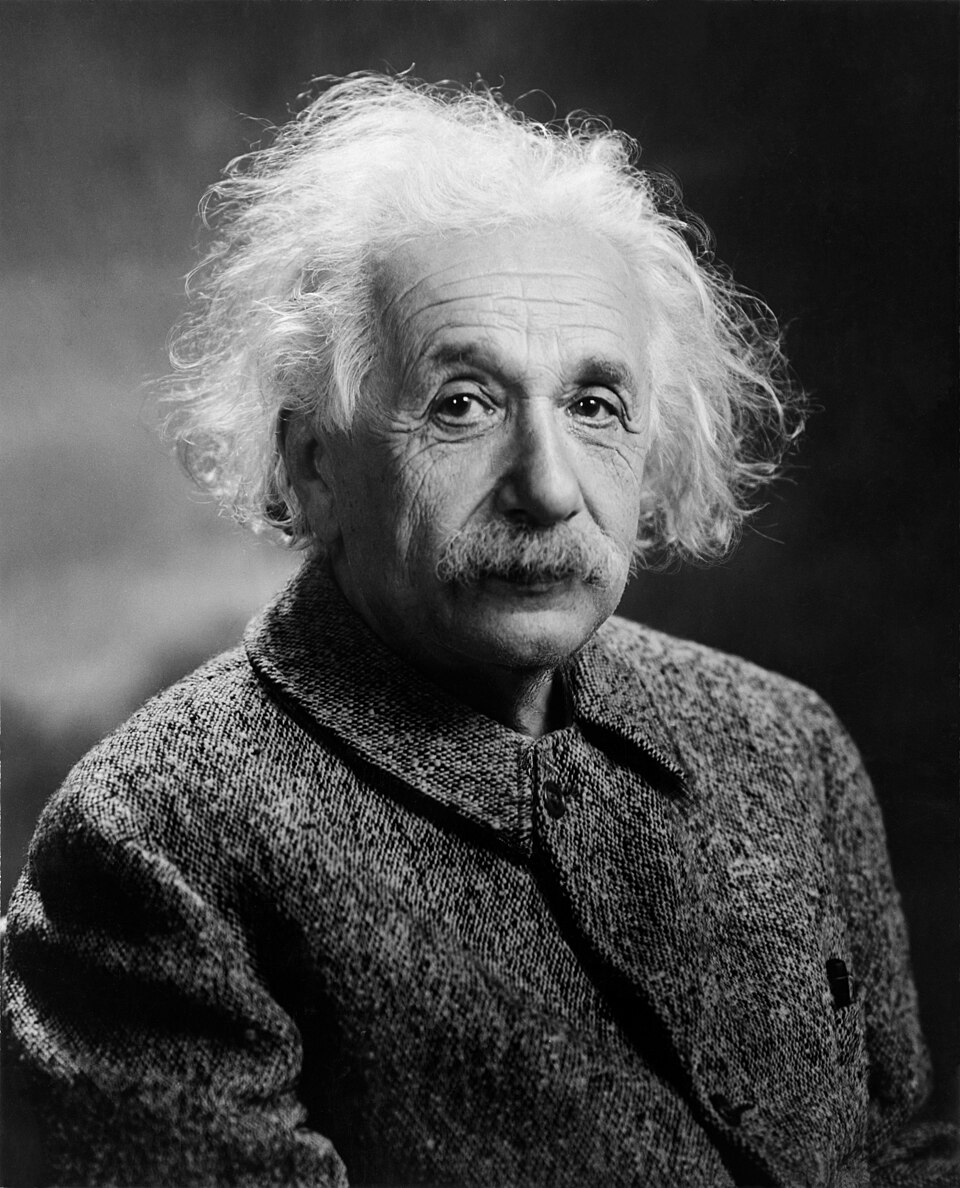
\includegraphics[width=0.6\textwidth]{pictures/cap6/einstein.jpeg}
    \caption{Albert Einstein (1879--1955). Con la Relatività Ristretta (1905), Einstein capovolse la domanda sul moto assoluto: anziché cercare un sistema di riferimento privilegiato, mostrò che le leggi della fisica sono le stesse in tutti i sistemi inerziali. La realtà fisica non risiede in un riferimento particolare, ma negli \textbf{invarianti}, vale a dire le quantità che si preservano passando da un riferimento all'altro. Fonte: \cite{wikipedia2024einstein}.}
    \label{fig:einstein}
\end{figure}
Ma se nessun sistema di riferimento è speciale, cosa è ``reale''? La risposta di Einstein fu precisa: sono reali gli \textbf{invarianti}, le quantità che restano identiche indipendentemente dal sistema di riferimento scelto. L'intervallo spaziotemporale $ds^2 = c^2\, dt^2 - dx^2 - dy^2 - dz^2$ cambia nelle sue componenti ($dt$, $dx$, $dy$, $dz$) quando si passa da un osservatore all'altro, ma la combinazione $ds^2$ resta la stessa. Lo spazio e il tempo, presi separatamente, sono relativi all'osservatore, come ombre sulla parete. L'intervallo $ds^2$, che li lega insieme, è l'oggetto fuori dalla caverna.
\subsubsection{Tre formulazioni, una sola fisica}
\label{subsubsec:tre_formulazioni}
La stessa lezione emerge in un contesto meno radicale ma altrettanto illuminante: le formulazioni della meccanica classica. Newton descrive il moto con forze e accelerazioni ($\vec{F} = m\vec{a}$); Lagrange riformula lo stesso contenuto fisico attraverso il principio di minima azione $S = \int_{t_1}^{t_2} L\, dt$; Hamilton introduce lo spazio delle fasi con posizione e momento coniugato $(q, p)$. Tre linguaggi matematici diversi. Tre ``rappresentazioni'' dello stesso sistema fisico. Una sola fisica.
Un sistema massa-molla, ad esempio, può essere descritto equivalentemente come:
\begin{itemize}
    \item Un'equazione differenziale: $m\ddot{x} = -kx$ \hfill (Newton)
    \item Un principio variazionale: $\delta \int \left(\tfrac{1}{2}m\dot{x}^2 - \tfrac{1}{2}kx^2\right) dt = 0$ \hfill (Lagrange)
    \item Un flusso nello spazio delle fasi: $\dot{q} = \tfrac{\partial H}{\partial p},\; \dot{p} = -\tfrac{\partial H}{\partial q}$ \hfill (Hamilton)
\end{itemize}
Nessuna di queste formulazioni è ``quella vera''. Le leggi vere sono quelle che si preservano nel passaggio da una formulazione all'altra: la frequenza di oscillazione $\omega = \sqrt{k/m}$, l'energia conservata, la periodicità del moto.
\subsubsection{Applicazione al dominio del significato}
\label{subsubsec:applicazione_significato}
Il parallelo con il problema delle rappresentazioni semantiche è diretto. La rappresentazione densa (embedding), la rappresentazione sparsa (attivazioni SAE) e la rappresentazione umana (struttura concettuale) sono tre ``formulazioni'' dello stesso oggetto, vale a dire il significato. Chiedersi quale sia quella vera è come chiedersi se la meccanica ``vera'' sia quella di Newton o quella di Lagrange: la domanda è mal posta.
La domanda corretta, suggerita dalla lezione della fisica, è un'altra:
\begin{quote}
\textit{Esistono invarianti semantici che si preservano attraverso tutte le rappresentazioni del significato? Se sì, questi invarianti, e non le rappresentazioni, sono le leggi fondamentali del significato.}
\end{quote}

\subsubsection{La Platonic Representation Hypothesis}
\label{subsubsec:platonic_rep}
La direzione di ricerca delineata nel paragrafo precedente, vale a dire cercare invarianti anziché rappresentazioni privilegiate, trova un supporto empirico significativo in un recente position paper presentato a ICML 2024.
In~\parencite{huh2024platonic} viene formulata la \textit{Platonic Representation Hypothesis}: reti neurali diverse, addestrate con obiettivi diversi su dati e modalità diverse, stanno convergendo verso un \textbf{modello statistico condiviso della realtà} nei loro spazi di rappresentazione.
L'intuizione è quella illustrata in Figura~\ref{fig:platonic_rep}: il mondo reale ($Z$) può essere osservato attraverso modalità diverse, un'immagine ($X$), una descrizione testuale ($Y$), un suono, un'equazione. Ciascuna modalità è una proiezione parziale della stessa realtà sottostante, esattamente come le ombre sulla parete della caverna platonica. La tesi proposta in~\parencite{huh2024platonic} è che gli algoritmi di rappresentazione, quando diventano sufficientemente potenti, recuperano la struttura condivisa che sta \textit{dietro} a tutte queste proiezioni.
\begin{figure}[htbp]
    \centering
    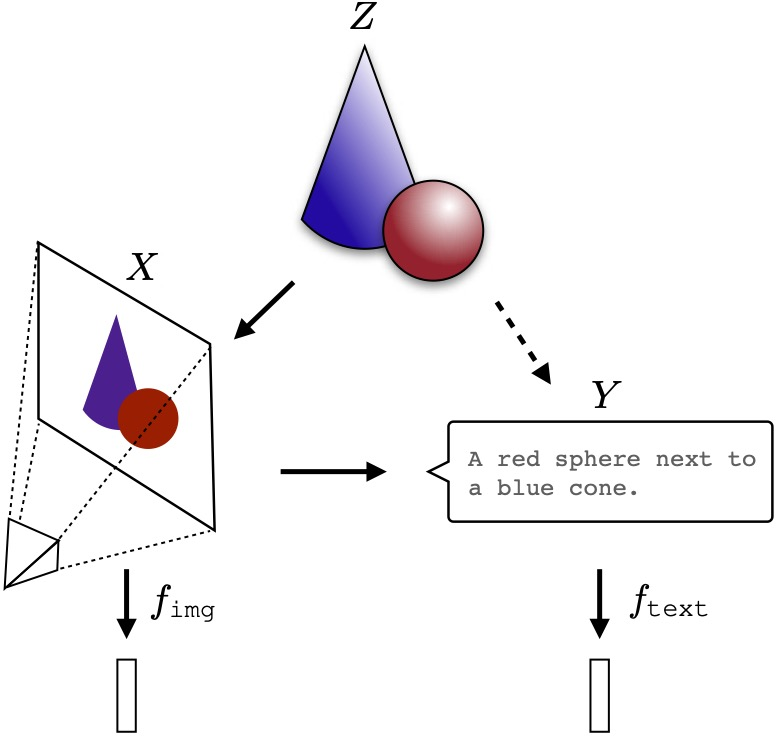
\includegraphics[width=0.65\textwidth]{pictures/cap6/platonic_rep_less_space_v2.jpg}
    \caption{La Platonic Representation Hypothesis, da~\parencite{huh2024platonic}. La realtà sottostante ($Z$), qui una sfera rossa accanto a un cono blu, genera proiezioni in modalità diverse: un'immagine ($X$) e una descrizione testuale ($Y$). Due encoder indipendenti, $f_{\text{img}}$ e $f_{\text{text}}$, trasformano queste proiezioni in rappresentazioni vettoriali. L'ipotesi è che, all'aumentare della scala e della generalità dei modelli, queste rappresentazioni convergano verso la stessa struttura, vale a dire il modello statistico della realtà $Z$.}
    \label{fig:platonic_rep}
\end{figure}

\subsubsection{Le evidenze}
\label{subsubsec:evidenze}
Le evidenze riportate in~\parencite{huh2024platonic} operano su tre livelli di convergenza:

\begin{enumerate}
    \item \textbf{Convergenza intra-modale.} Analizzando 78 modelli di visione, gli autori mostrano che quelli più performanti hanno rappresentazioni sempre più allineate tra loro. I modelli deboli divergono ognuno a modo suo; quelli forti si assomigliano tutti, un fenomeno che viene denominato, parafrasando Tolstoj, lo ``scenario Anna Karenina'': \textit{tutti i buoni modelli sono uguali; ogni cattivo modello è cattivo a modo suo}.
    \item \textbf{Convergenza cross-modale.} Modelli di linguaggio (solo testo) e modelli di visione (solo immagini), mai addestrati congiuntamente, mostrano strutture di similarità sempre più allineate all'aumentare della scala. La distanza tra ``cono'' e ``sfera'' nello spazio di un LLM correla con la distanza tra le immagini corrispondenti nello spazio di un modello di visione, e questa correlazione cresce con la capacità di entrambi.
    \item \textbf{Convergenza verso il cervello.} I modelli di visione più performanti sono anche quelli più allineati con le risposte neuronali misurate nel cervello umano tramite fMRI. La convergenza non avviene solo tra macchine: avviene tra macchine e biologia.
\end{enumerate}

\subsubsection{Cosa guida la convergenza?}
\label{subsubsec:guida_convergenza}
In~\parencite{huh2024platonic} vengono identificate tre pressioni selettive. La prima è la \textit{generalità dei task}: più compiti un modello deve risolvere, meno rappresentazioni li soddisfano tutti simultaneamente; al limite, ne resta una sola. La seconda è la \textit{capacità del modello}: modelli più grandi catturano più struttura statistica dei dati, convergendo verso quella reale. La terza è il \textit{simplicity bias}: le reti neurali hanno un bias implicito verso soluzioni semplici, e la rappresentazione ``platonica'' è, in un senso preciso, la più semplice che cattura fedelmente la realtà.
\subsubsection{Come si misura la convergenza?}
\label{subsubsec:misura_convergenza}
Un aspetto metodologico cruciale del lavoro presentato in~\parencite{huh2024platonic} è la scelta di caratterizzare le rappresentazioni attraverso i loro \textbf{kernel}, vale a dire la struttura di distanze e similarità tra i punti. Due rappresentazioni sono considerate ``la stessa'' se i loro kernel sono uguali: se, per ogni coppia di input, il grado di similarità misurato da una rappresentazione è proporzionale a quello misurato dall'altra.
Formalmente, se un encoder testuale $f_{\text{text}}$ è allineato con un encoder visivo $f_{\text{img}}$, allora:
\begin{equation}
    \text{sim}\big(
        f_{\text{text}}(\text{``cono''}),
        f_{\text{text}}(\text{``sfera''})
    \big)
    \;\approx\;
    \text{sim}\big(
        f_{\text{img}}(\triangle),
        f_{\text{img}}(\circ)
    \big)
    \label{eq:kernel_alignment}
\end{equation}
In altri termini: ciò che è invariante tra rappresentazioni diverse è la \textit{struttura relazionale}, non i vettori in sé, ma le distanze tra di essi. È esattamente l'analogo dell'intervallo spaziotemporale $ds^2$ di Einstein: le coordinate cambiano, le distanze si preservano.
\subsubsection{Il collegamento con PRISMA}
\label{subsubsec:collegamento_prisma}
La connessione con il presente lavoro è diretta. Le feature families estratte da PRISMA, \textit{Time in physics} con i suoi 47 children, \textit{Ising model} con le sue correlazioni con \textit{Phase Transitions} e \textit{Quantum Spin}, sono una manifestazione esplicita di questa struttura relazionale.
Se la Platonic Representation Hypothesis è corretta, allora le stesse famiglie, le stesse gerarchie, le stesse relazioni di co-attivazione dovrebbero emergere indipendentemente dal modello di embedding scelto, dal corpus utilizzato e persino dalla modalità dei dati.
PRISMA, in questa prospettiva, non è solo uno strumento di interpretabilità: è un \textbf{traduttore} che rende la struttura platonica leggibile, trasformando pattern statistici opachi in concetti nominabili e relazioni navigabili.
\subsubsection{La proposta: cercare isomorfismi tra rappresentazioni}
\label{subsubsec:proposta_isomorfismi}
La convergenza osservata in~\parencite{huh2024platonic} tra modelli diversi suggerisce l'esistenza di una struttura semantica sottostante, la ``realtà platonica'' del significato. Ma il framework proposto in quel lavoro confronta rappresentazioni dense tra loro (BERT~\parencite{devlin2018bert} vs.\ DINOv2 vs.\ LLaMA), restando nello spazio dei kernel: la struttura condivisa è rilevata statisticamente, ma rimane opaca, vale a dire non è noto \textit{quali} concetti si preservino, solo che \textit{qualcosa} si preserva.
PRISMA aggiunge un elemento cruciale: lo Sparse Autoencoder come \textbf{strumento di traduzione} che rende la struttura esplicita. Nella rappresentazione sparsa, gli invarianti non sono solo pattern astratti di distanza tra vettori, ma concetti \textit{nominabili}, famiglie semantiche, gerarchie interpretabili. La feature \textit{Time in physics} e i suoi 47 children non sono un pattern statistico opaco: sono una struttura tassonomica che un fisico riconoscerebbe immediatamente.
La direzione di ricerca che questo lavoro propone è dunque la seguente: anziché cercare una rappresentazione semantica privilegiata, un ``etere del significato'', concentrarsi su ciò che \textbf{non varia} quando si passa da una rappresentazione all'altra. Formalmente, cercare \textbf{isomorfismi} tra le tre rappresentazioni (densa, sparsa, umana) e caratterizzare gli invarianti che questi isomorfismi preservano. Due domande strutturano questo programma.
La prima è una domanda tecnica, alla quale è possibile rispondere empiricamente: \textbf{denso e sparso sono isomorfi?} Se l'errore di ricostruzione $\vec{\epsilon}$ è trascurabile, come in Eq.~\ref{eq:reconstruction}:
\begin{equation}
    \vec{x}_{\text{denso}} = W_{\text{decode}} \cdot \vec{x}_{\text{sparso}} + \vec{\epsilon}, \quad \text{con} \quad \|\vec{\epsilon}\| \approx 0
    \label{eq:reconstruction}
\end{equation}
allora le due rappresentazioni sono isomorfe, e la matrice $W_{\text{decode}}$ è la funzione di traduzione. Gli SAE attuali hanno errori piccoli ma non nulli: sono \textit{quasi} isomorfi. L'informazione contenuta nel residuo $\vec{\epsilon}$ è una domanda aperta: potrebbe essere rumore, oppure struttura semantica non monosemantica che sfugge alla decomposizione sparsa.
La seconda è la domanda filosoficamente decisiva: \textbf{sparso e umano sono isomorfi?} Se le feature monosemantiche estratte dal SAE corrispondono ai concetti atomici della cognizione umana, se le famiglie semantiche di PRISMA rispecchiano le categorie con cui viene organizzato il mondo, allora le reti hanno \textit{scoperto} la struttura della mente umana. Se non corrispondono, le possibilità sono tre: o la cognizione umana possiede concetti che le reti non catturano, o le reti hanno ``concetti'' che la cognizione umana non possiede, oppure, la possibilità più interessante, entrambe approssimano qualcosa di terzo: la struttura platonica sottostante, di cui sia la mente umana sia la rete neurale sono proiezioni imperfette.
\subsubsection{Candidati invarianti semantici}
\label{subsubsec:candidati_invarianti}
Se gli invarianti semantici esistono, quali strutture concrete potrebbero preservarsi attraverso rappresentazione densa, sparsa e umana?
Un primo candidato naturale sono le \textbf{relazioni di analogia}. Se ``re meno uomo più donna uguale regina'' vale nello spazio degli embedding come aritmetica vettoriale, nello spazio sparso come pattern di co-attivazione di feature, e nella mente umana come giudizio intuitivo di relazione, allora quella relazione è un invariante: non appartiene a nessuna rappresentazione in particolare, ma le attraversa tutte.
Un secondo candidato sono le \textbf{strutture gerarchiche}. Se ``cane è un mammifero'' si preserva in tutte le rappresentazioni, come relazione di inclusione geometrica nello spazio denso, come relazione parent-child nel grafo delle feature families nello spazio sparso, come categorizzazione spontanea nella cognizione umana, allora la gerarchia tassonomica è un invariante. Le 590 famiglie estratte da PRISMA, con la loro organizzazione a stella (parent generale, children specifici), sono candidati particolarmente interessanti: se le stesse famiglie emergono da modelli diversi, su dati diversi, con SAE diversi, allora la struttura di famiglia non è un artefatto del metodo, ma una proprietà del dominio.
Un terzo candidato sono gli \textbf{ordini di similarità}: se $\text{sim}(A, B) > \text{sim}(A, C)$ in tutte le rappresentazioni, se ``cono'' è più vicino a ``sfera'' che a ``trattore'' ovunque la si misuri, allora quell'ordinamento è un invariante. È esattamente ciò che viene misurato in~\parencite{huh2024platonic} attraverso il kernel alignment, e il fatto che la convergenza tra modelli cresca con la scala è un'evidenza indiretta che questi ordinamenti tendono a stabilizzarsi.
Infine, un candidato più sottile ma potenzialmente più profondo è la \textbf{dimensionalità effettiva} dello spazio semantico. L'analisi dell'Effective Rank presentata nel Paragrafo~\ref{subsec:effective_rank_results} ha mostrato che la struttura semantica comprime le rappresentazioni in modo sistematico: il Semantic Compression Ratio cresce monotonicamente con l'expansion factor, raggiungendo il 59,9\% per $\rho = 64$. Se questa compressione è una proprietà della struttura del significato e non della rappresentazione specifica, allora l'SCR stesso potrebbe essere un invariante: una misura di quanto il dominio semantico ``è comprimibile'', indipendentemente da come lo si rappresenta.
\subsubsection{Il ruolo dell'Effective Rank e dell'SCR}
\label{subsubsec:ruolo_er_scr}
L'Effective Rank e il Semantic Compression Ratio introdotti in questo lavoro potrebbero servire come strumenti quantitativi per lo studio di questi invarianti. In particolare, se la compressione semantica è una proprietà della struttura del significato e non della rappresentazione specifica, allora l'SCR dovrebbe essere \textbf{invariante rispetto al modello di embedding} utilizzato.
Un esperimento cruciale per sviluppi futuri sarebbe il seguente: ripetere l'analisi dell'Effective Rank del Paragrafo~\ref{subsec:effective_rank_results} utilizzando modelli di embedding diversi (BERT~\parencite{devlin2018bert}, GPT, modelli multilingue, modelli multimodali) sullo stesso corpus. Se l'SCR converge verso valori simili, vale a dire se la semantica comprime le rappresentazioni nella stessa misura indipendentemente da come sono state costruite, allora l'SCR stesso è un candidato invariante semantico, una proprietà del dominio e non del modello.
Questo collegherebbe direttamente il contributo tecnico della presente tesi (l'analisi ER/SCR) con il programma di ricerca più ampio sugli invarianti, fornendo una metrica operativa per testare la Platonic Representation Hypothesis nel contesto degli Sparse Autoencoder.
\subsubsection{Visione d'insieme}
\label{subsubsec:visione_insieme}
Questo lavoro è partito da un problema tecnico: le rappresentazioni dense dei modelli linguistici sono opache, e l'interpretabilità richiede strumenti capaci di rendere esplicita la struttura che esse codificano. Lo Sparse Autoencoder, applicato agli embedding densi, si è rivelato uno strumento efficace: estrae concetti interpretabili, li organizza in famiglie gerarchiche coerenti con le tassonomie dei domini di applicazione, e produce rappresentazioni la cui dimensionalità effettiva riflette in modo quantificabile la struttura semantica sottostante.
Ma nel costruire questo strumento, è emerso qualcosa di più ampio del problema tecnico di partenza. Le feature estratte da PRISMA non sono artefatti del metodo: sono strutture che un esperto di dominio riconosce immediatamente, \textit{Time in physics} e i suoi 47 children, \textit{Ising model} con le sue correlazioni con \textit{Phase Transitions} e \textit{Quantum Spin}, le famiglie cliniche che rispecchiano la logica del ragionamento pediatrico. La consistenza di queste strutture tra domini completamente diversi, fisico e clinico, suggerisce che l'organizzazione gerarchica non è imposta dal SAE, ma \textit{rivelata} da esso.
La Platonic Representation Hypothesis formulata in~\parencite{huh2024platonic} offre una cornice teorica per questa osservazione: se modelli diversi, addestrati su dati e modalità diverse, convergono verso la stessa struttura relazionale, allora quella struttura non appartiene a nessun modello in particolare, ma appartiene al dominio. E se la stessa struttura si ritrova anche nella cognizione umana, come le evidenze neuroscientifiche cominciano a suggerire, allora è possibile trovarsi di fronte a qualcosa che somiglia a una legge: un invariante del significato, indipendente dalla rappresentazione che lo codifica.

Non è ancora noto se gli invarianti semantici esistano in senso forte, vale a dire se esista, fuori dalla caverna, una struttura del significato formalizzabile come le simmetrie della fisica. Ma è noto che, quando si costruiscono strumenti capaci di tradurre tra rappresentazioni diverse, le stesse strutture riemergono. E il Semantic Compression Ratio, la misura di quanto la semantica comprime lo spazio delle rappresentazioni, cresce monotonicamente con la capacità del SAE, raggiungendo il 59,9\% per $\rho = 64$: la struttura del significato non solo esiste, ma è quantificabile.
\begin{notebox}
\textbf{Da PRISMA alla ricerca degli invarianti}\\[0.5em]
Il presente lavoro ha costruito uno strumento, lo Sparse Autoencoder applicato a embedding densi, e ha mostrato che funziona: estrae concetti interpretabili, organizzati in famiglie gerarchiche, la cui struttura comprime sistematicamente lo spazio delle rappresentazioni.
La direzione futura è usare questo strumento non come fine, ma come \textit{mezzo}: un traduttore tra rappresentazioni che rende esplicita la struttura semantica, permettendo di cercare ciò che rimane invariante attraverso tutte le traduzioni possibili.
Se tali invarianti esistono e sono formalizzabili, essi costituiscono le leggi fondamentali del significato, gli ``atomi semantici'' che nessuna rappresentazione particolare crea, ma che tutte, necessariamente, riflettono.
\end{notebox}